\chapter[APÊNDICE \ref{Ap:Cavity2}]{Análise de convergência no problema de cavidade bidimensional}
\label{Ap:Cavity2}

Para comparação da convergência entre os modelos implementados assumiu-se a cavidade apresentada no Apêndice \ref{Ap:Cavity}, onde, para no presente caso, realizou-se um simulação com $\Rey=1000$ partindo de uma condição inicial $\BB{u}=\BB{0}$ em todo o domínio. As medidas de resíduos observadas foram relacionadas à velocidade ($e_u=\norm{\Delta\BB{U}}$) e à pressão ($e_p=\norm{\Delta\BB{P}}$) e a simulação foi conduzida até que um resíduo abaixo de $1\times10^{-8}$ fosse obtido. A Figura \ref{fig:comp-res} apresenta a convergência dos modelos segundo essas medidas.

\begin{figure}[h!]
    \centering
    \caption{Comparação do resíduo da:}
    \begin{subfigure}{\textwidth}
        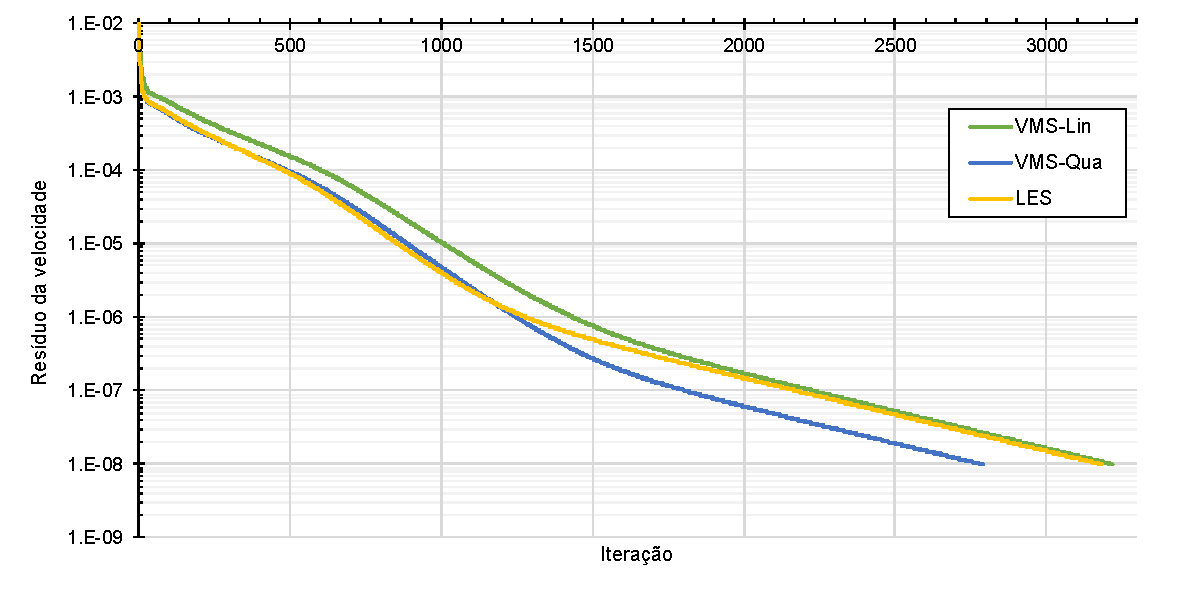
\includegraphics[width=\linewidth]{Figuras/Cavity/resvel.pdf}
        \caption{velocidade.}
    \end{subfigure}
    \begin{subfigure}{\textwidth}
        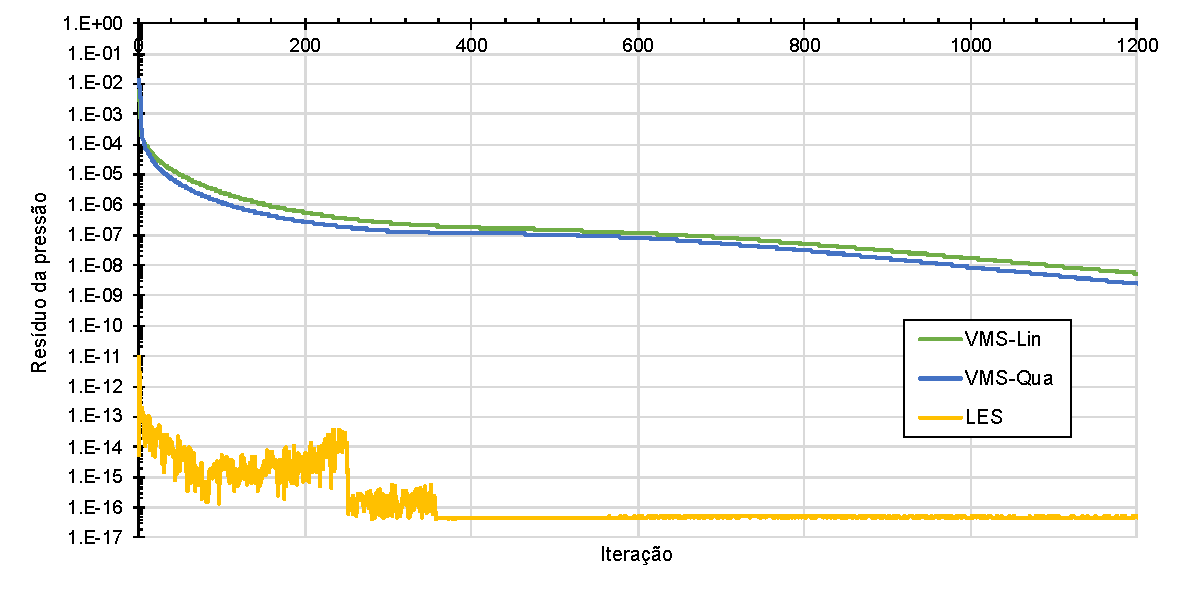
\includegraphics[width=\linewidth]{Figuras/Cavity/respre.pdf}
        \caption{pressão.}
    \end{subfigure}
    \\Fonte: Autoria Própria (\the\year).
    \label{fig:comp-res}
\end{figure}

Também foi observado o tempo necessário para que a convergência fosse atingida. A Tabela \ref{tab:comp-res} apresenta o número de iteração necessárias para que ambas as medidas de erro atingissem a tolerância, o tempo médio por iteração e o tempo total da simulação.

\begin{table}[h!]
    \centering
    \caption{Resultados do estudo de convergência dos métodos.}
    \begin{tabular}{lccc}
        \hline
        Modelo         & número de iterações & tempo por iteração (s) & tempo (min) \\\hline
        VMS linear     & 3218                & 0,650                  & 34,872      \\
        VMS quadrático & 2788                & 3,814                  & 177,260     \\
        LES            & 3182                & 3,494                  & 185,357     \\\hline
    \end{tabular}
    \\Fonte: Autoria Própria (\the\year).
    \label{tab:comp-res}
\end{table}

Observa-se no resíduo da velocidade que todos os métodos tiveram uma convergência mais rápida no início da simulação, pois um fluxo rotacional ainda estava sendo obtido pelos modelos. Após se estabelecer esse fluxo a convergência desacelerou até atingir a tolerância admitida. Já com relação ao resíduo da pressão verifica-se que o modelo LES obteve uma convergência imediata, no entanto a convergência dos demais modelos também foi rápida de tal forma a essa medida não ser o limitante em relação ao tempo de processamento. Ao final do processamento o VMS quadrático foi o que precisou da menor quantidade de iterações para convergir, no entanto, devido à quantidade de graus de liberdade ser maior, seu tempo requerido para cada iteração aumentou, necessitando de um tempo similar ao LES.